\documentclass[11pt,a4paper]{article}

% 日本語対応パッケージ
\usepackage[haranoaji]{luatexja}
\usepackage{luatexja-fontspec}
\usepackage{fontspec}

% 基本パッケージ
\usepackage{amsmath}
\usepackage{amsfonts}
\usepackage{amsthm}
\usepackage{amssymb}
\usepackage{graphicx}
\usepackage{hyperref}
\usepackage{geometry}
\usepackage{enumitem}
\usepackage{setspace}
\usepackage{algorithm}
\usepackage{algorithmic}
\usepackage{bm}

% ページ設定
\geometry{margin=2.5cm}
\setlength{\parindent}{0pt}
\setlength{\parskip}{6pt}

\newtheorem{proposition}{Proposition}

\title{2022年2月 ノイズに頑健な協調距離軽量学習\_松井諒生}
\author{吉村光瑛}
\date{2025年7月18日}

\begin{document}

\maketitle

\begin{abstract}
  昨今,「推薦システム」の研究が盛んに行われている.推薦システムとは個人個人にとってのモノや情報の価値を特定することを目的とした情報検索・機械学習の一分野である.例えば,web サービスにおいてユーザーの行動履歴から潜在的な嗜好性を学習し,各ユーザーのニーズに合ったコンテンツを「おすすめ」として表示することなどが挙げられる.特に web サービスにおける推薦システムでは,1) ユーザーの嗜好性を学習する際に implicit feedback と呼ばれるユーザーの積極的な行動を必要としないデータを利用する,2) ユーザーの嗜好性を予測・推論する際にユーザーとアイテムの埋め込みベクトルを利用する,という2点が要求される.近年では,後者の要求に応える手法として協調距離計量学習 (Collaborative Metric Learning, CML) と呼ばれる手法が発展してきた.しかし,この手法は前者の要求である implicit feedback に起因するノイズラベル問題に対応していない.そこで本研究では,CML の学習においてノイズを網羅的に扱い,効果的に対処する方法を提案する.実験の結果,提案手法は既存手法と比較して 2 つの要求に対する性能が大幅に改善することがわかった.
\end{abstract}

\section*{第一章 序論}

\subsection*{1.1 webサービスの要求を満たす推薦システムの特徴}
webサービスにおける推薦システムでは主に2つの要求がされる。

1つ目の要求は、ユーザーおよびアイテムの嗜好性や類似性を学習する際にimplicit feedbackデータを利用する点。今日のwebサービスにおいてユーザーの嗜好を表す情報として取得・利用できるデータはexplicit feedbackとimplicit feedbackの2つ。implicit feedbackはユーザーへの調査協力を必要としないため、\textbf{explicit feedbackと比較してデータ収集コストが小さい}というメリットがある。しかし、\textbf{クリックや閲覧などの行動が必ずしもユーザーの嗜好を表すとは限らない}ため、データに含まれるノイズは比較的大きい。近年のWebサービスではログ技術やビッグデータ処理技術が発展してきているため、ユーザーの能動的な行動を必要としないimplicit feedbackのデメリットを考慮したノイズに頑健な推薦システムの構築を目指す研究が盛んにおこなわれている。

\begin{table}[h]
  \centering
  \begin{tabular}{c||cc}
    & explicit feedback & implicit feedback \\
    \hline
    \hline
    データ収集の方法 & レビュー・アンケート & 閲覧/クリックの履歴 \\ 
    ユーザーの態度 & 積極的 & 消極的 \\
    データ内のノイズ & 少ない & 多い \\
    データ収集コスト & 大きい & 小さい \\    
  \end{tabular}
  \caption{ユーザーの嗜好に関する2種類のデータとその特徴}
\end{table}

主にimplicit feedbackに起因するノイズは2つに分けられる。1つ目のノイズは、ユーザーがあるアイテムにクリックしたものの、実際にはそのアイテムに興味がなかったという事象を指す\textbf{ポジティブノイズ(偽陽性)}。このようなノイズは、ユーザーのクリック成否がタイトルや説明文の第一印象に左右されやすいことが原因とされる。2つ目のノイズは、ユーザーが自身の嗜好に合ったアイテムを見逃している事象を指す\textbf{ネガティブノイズ(偽陰性)}である。このノイズを無視して行うと、単に過去にクリックしたアイテムのみを推薦してしまう。

\begin{itemize}
  \item ポジティブノイズ(偽陽性)
  \begin{itemize}
    \item ユーザーがあるアイテムにクリックしたものの、実際にはそのアイテムに興味がなかったという事象
    \item ユーザーのクリック成否がタイトルや説明文の第一印象に左右されやすいことが原因とされる
  \end{itemize}
  \item ネガティブノイズ(偽陰性)
  \begin{itemize}
    \item ユーザーが自身の嗜好に合ったアイテムを見逃している事象
    \item このノイズを無視して行うと、単に過去にクリックしたアイテムのみを推薦してしまう
  \end{itemize}
\end{itemize}

2つ目の要求は、ユーザーおよびアイテムの嗜好性や類似性を予測・推論する際に埋め込みベクトルを利用する点である。埋め込みベクトルとは、観測した(ユーザー - アイテム)間の関係性データをもとに、ユーザーおよびアイテムをそれぞれ1つのベクトルとして表現したものである。そして、ユーザーおよびアイテムの潜在的な嗜好や類似性をそのベクトルの類似度によって推定する。この埋め込みベクトルを利用するメリットは主に2つある。1つ目のメリットは\textbf{低遅延性}である。現代Webサービスは大量のユーザーに瞬時にサービスを提供する必要がある。\textbf{埋め込みベクトルを利用すると、近似近傍探索などの手法を用いることで、ユーザーベクトルに類似したアイテムのベクトルを、ユーザー体験の毀損が起きない時間内で発見することが可能}である。これにより、全てのアイテムについて嗜好性を計算することを回避したうえで、膨大なアイテム群の中から推薦すべきアイテムを発見できる。2つ目のメリットは、\textbf{(ユーザー - ユーザー)間および(アイテム - アイテム)間の類似度も表現できる}という点である。ユーザーおよびアイテムを埋め込みベクトルとして表現することによって、ユーザーの潜在的な嗜好に合ったアイテムを捉えるだけでなく、ユーザーと潜在的に類似したユーザや、アイテムと潜在的に類似した別のアイテムを捉えることも可能になる。実務的なインパクトとしては、顧客セグメントを捉えるマーケティングへの応用、SNSにおける友達の推薦、ECサイトにおける関連商品・代替商品の推薦などがある。

\begin{itemize}
  \item 低遅延性
    \begin{itemize}
      \item 現代Webサービスは大量のユーザーに瞬時にサービスを提供する必要がある
      \item 埋め込みベクトルを利用すると、近似近傍探索などの手法を用いることで、ユーザーベクトルに類似したアイテムのベクトルを、ユーザー体験の毀損が起きない時間内で発見することが可能
    \end{itemize}
  \item (ユーザー - ユーザー)間および(アイテム - アイテム)間の類似度の表現
    \begin{itemize}
      \item ユーザーの潜在的な嗜好に合ったアイテムを捉えるだけでなく、ユーザーと潜在的に類似したユーザや、アイテムと潜在的に類似した別のアイテムを捉えることも可能
      \item 実務的なインパクトは、顧客セグメントを捉えるマーケティングへの応用、SNSにおける友達の推薦、ECサイトにおける関連商品・代替商品の推薦など
    \end{itemize}
\end{itemize}

ここまでをまとめると,web サービスにおける推薦システムの構築にあたって 2 つの要求に応えるには \textbf{implicit feedback に起因するポジティブノイズおよびネガティブノイズの両者に対処した上で,(ユーザー – アイテム) 間のみならず (ユーザー – ユーザー) 間および (アイテム – アイテム) 間の関係性を高速かつ正確に捉えられる埋め込みベクトルを学習する必要がある.}

\subsection*{1.2 協調距離計量学習}

以下の2つの性質を持つ埋め込みベクトルを獲得できるアルゴリズムを開発すればよい。

性質1 implicit feedbackに起因する以下2つのノイズに頑健
\begin{itemize}
  \item ポジティブノイズ(偽陽性)
  \item ネガティブノイズ(偽陰性)
\end{itemize}

性質2 以下3つの全ての関係を精緻に捉えられる
\begin{itemize}
  \item (ユーザー - アイテム)間
  \item (ユーザー - ユーザー)間
  \item (アイテム - アイテム)間
\end{itemize}

性質2を満たすために、協調距離軽量学習(Collaborative Metric Learning, CML)と呼ばれるアルゴリズムを拡張していく。CMLは、埋め込みベクトルを用いた最も標準的なアルゴリズムである\textbf{行列分解が、(ユーザー - ユーザー)間と(アイテム - アイテム)間の細かな関係性を表現できていない}という指摘[23, 24]を受けて開発された。行列分解がユーザーとアイテムを表す類似度関数としてベクトルの内積を用いているのと対照的に、CMLは類似度関数としてユークリッド距離を採用している。距離関数は三角不等式の関係性を満たすため、(ユーザー - アイテム)間の関係性データのみから学習しても、(ユーザー - ユーザー)間および(アイテム - アイテム)間の関係性を捉えることができる。

ただし、最も素朴なCMLはimplicit feedbackのノイズに対処していない。Tranら[31]はCMLの学習において部分的にノイズラベル問題へ取り組んだ。

CMLについて
\begin{itemize}
  \item ユーザー$u$およびユーザー$u$とのインタラクションを観測したアイテム$i$(ポジティブアイテム)、ユーザー$u$とのインタラクションを観測していないアイテム$j$(ネガティブアイテム)を加えたトリプレット$(u, i, j)$を構成単位とした損失関数
  \item トリプレットを一様ランダムに抽出し、勾配降下法によるパラメータ更新を繰り返すことによって埋め込みベクトルを学習
    \begin{itemize} 
      \item 一様ランダムなサンプリングでは一定確率でノイズなデータを含んでしまうため、学習が非効率な問題がある
      \item Tranらはこの問題を解決するためにデータの信頼度で重みづけした2段階のサンプリングによってノイズの少ないネガティブアイテム$i_n$を抽出する方法を提案
    \end{itemize}
\end{itemize}

しかし、ここまでの研究には依然として2つの課題が残されている。

まず1つ目の課題は、CMLにおいて重み付けのサンプリングが十分でない可能性がある点である。重みづけによってノイズのあるネガティブアイテムが抽出される確率が減らされるかもしれないが、三角不等式の性質上、1度でもノイズのあるデータがサンプリングされると、ノイズの影響が全体的に広がってしまう。ゆえに、\textbf{極めてノイズのあるデータはデータセットから削除するクリーニングと呼ばれるアプローチも検証すべき}である。

2つ目の課題は、ポジティブアイテム$i$についてのノイズを考慮していない点である。

この2つの課題を解決するため、この研究ではCMLの学習前にデータの信頼度を推定し、ポジティブ・ネガティブの両ノイズに対処した重みづけまたはクリーニングに活用する方法を提案する。信頼度の推定には、ノイズなラベルを含んだ画像分類における最高水準手法である信頼学習(Confident Learning)を参考にする。

\begin{figure}[h]
  \centering
  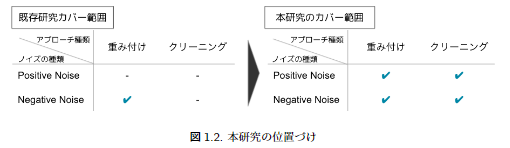
\includegraphics[width=0.8\textwidth]{本研究の位置づけ.png}
  \caption{この研究の位置づけ}
\end{figure}

そして、

\begin{itemize}
  \item 提案手法は既存手法と比較してノイズに頑健に (ユーザー–アイテム) 間の関係性を捉え,より正確な推薦を行うことは可能か.(性質 1 かつ性質 2-a に対する性能改善)
  \item 提案手法は既存手法よりもノイズに頑健に (ユーザー–ユーザー) 間,(アイテム–アイテム) 間の関係性を捉えることは可能か.(性質 1 かつ性質 2-b,2-c に対する性能改善)
\end{itemize}

これらをリサーチクエッションとして設定する。ここでのノイズはimplicit feedbackに起因するポジティブノイズとネガティブノイズを指す。

\section*{第二章 関連研究}

\subsection*{2.2 implicit feedbackと埋め込みベクトルによる推薦システム}

\subsubsection*{2.2.1行列分解(MF)}

最も標準的な推薦システムは行列分解をベースとした協調フィルタリングであると言えるぐらいメジャーな手法。行にユーザー、列にアイテム、要素に各ユーザーアイテムペアの評価値$Y_{u,i}$を持つ行列 $Y \in \mathbb{R}^{N_U \times N_I}$について、
$$
	Y \approx U \cdot V
$$
のように2つの低ランク行列 $U \subset \mathbb{R}^{N_U \times l}$、$V \subset \mathbb{R}^{l \times N_I}$ の積で近似するアルゴリズムである。ただし、$l$は近似するランク数を表す。この行列 $U,V$は、最適化問題
$$
	U, V = \underset{U, V}{\arg \min} \| Y - U \cdot V \|^2_F
$$
を解くことで達成される。$\| \cdot \|_F$はフロベニウスノルムを表す。これによって求めた$U, V$ を用いて $\hat{Y} = U \cdot V$ を再構築することで、潜在的な評価値行列 $\hat{Y}$を獲得できる。そして、この $\hat{Y}$ をもとにユーザーに対して評価の高いアイテムを推薦することが可能となる。

要素ごとの近似として表現すると、次のようになる。

$$
  \underset{\Theta}{\min} \sum_{u \in \mathcal{U}} \sum_{i \in \mathcal{I}} \cdot (Y_{u,i} - \hat{Y_{u,i}})^2, \quad \text{where} \; \hat{Y_{u,i}} = \mathbf{v_u^T} \mathbf{v_i}
$$

また、ユーザーベクトルおよびアイテムベクトルの内積によって関係性・評価値を表していることから、**類似度関数を $Sim(u, i) = \mathbf{v_u^T} \mathbf{v_i}$ として考えている手法だと見なせる。

\subsubsection*{2.2.2 重み付き行列分解(WMF)}

しかし、単純な行列分解は$Y_{u,i}$のノイズを考慮していない。Huらは$Y_{u,i}$の信頼性$c_{u,i}$で重み付き行列分解(Weighted MF)を以下のように定式化した。

$$
  \underset{\Theta}{\min} \sum_{u \in \mathcal{U}} \sum_{i \in \mathcal{I}} c_{u,i} \cdot (Y_{u,i} - \hat{Y_{u,i}})^2, \quad \text{where} \; \hat{Y_{u,i}} = \mathbf{v_u^T} \mathbf{v_i}
$$

$c_{u,i}$は任意に設定が可能である。

\subsubsection*{2.2.3 Bayesian Personalized Ranking(BPR)}

Rendleらはランキング学習によるimplicit feedbackを用いた推薦システムの構築方法を提案した[8]。一般に推薦システムでは、あるユーザーが到来した際、各アイテムとの類似度を計算し、最も類似度の高いアイテムをいくつか推薦する。このとき、類似度は評価値そのものを表現している必要はない。そのため、インタラクションのあった$Y_{u,i} = +1$であるユーザーアイテムペア$(u,i)$の類似度がインタラクションのない$Y_{u,j} = -1$であるユーザーアイテムペア$(u,j)$の内積よりも相対的に大きくなるよう埋め込みベクトルの学習を行うランキング学習を導入した。特に、
$$
  \sum_{(u,i) \in \mathcal{S}} \sum_{j \in \mathcal{D}_u} \log \sigma(\mathbf{v_u^T} \mathbf{v_j} - \mathbf{v_u^T} \mathbf{v_i}) + \lambda \left( \sum_{u \in \mathcal{U}} \| \mathbf{v_u} \|^2 + \sum_{i \in \mathcal{I}} \| \mathbf{v_i} \|^2 \right)
$$
を最小化することで埋め込みベクトルを学習する。ただし、$\sigma$はシグモイド関数$\sigma(x) = \frac{1}{1 + e^{-x}}$を表し、$\lambda$は正則化の強さを表す。式より、ユーザー$u$に対してインタラクションのあったアイテム$i$との内積を大きく、インタラクションのないアイテム$j$との内積を小さくすることが出来る。これによって、推薦システムそのものの目的に対して直接的な学習ができるため、推薦の性能が向上する。

\subsubsection*{2.2.4 協調距離軽量学習(CML)}

上記の行列分解やBPRは埋め込みベクトルの内積によって、ユーザーとアイテムの潜在的な嗜好性を予測している。しかし、Hsiecらは\textbf{ユーザーベクトル同士、アイテムベクトル同士の内積はそれらの関係性の強さを表しておらず、この性質が推薦の精度や埋め込みベクトルの解釈性、拡張性に大きな影響を与えている}ことを指摘した[21]。

この問題を解決するために同研究で提案された手法が、協調距離軽量学習(Collaborative Metric Learning, CML)である。CMLは損失関数を
$$
  \mathcal{L}^{\text{cml}}(\Theta) = \sum_{(u,i) \in \mathcal{S}} \sum_{j \in \mathcal{D}_u} [1 + d(\mathbf{v_u}, \mathbf{v_i})^2 - d(\mathbf{v_u}, \mathbf{v_j})^2]_+
$$
と定義する。ここで、$d$はユークリッド距離、$[]_+$は関数$[x]_+ = \min\{ 0, x \}$を表す。$d$がCMLにおける類似度関数となる。つまり、CMLはインタラクションのあった(ユーザー - アイテム)間の距離を近づけ、インタラクションのない(ユーザー - アイテム)間の距離を遠ざけるような目的関数を持つ。\textbf{類似度関数に距離関数を用いる点がBPRとの大きな相違点}である。距離関数の三角不等式の性質を用いると、
$$
  d(u_1, i_1) + d(u_2, i_2) \geq d(u_1, i_2) + d(u_2, i_1)
$$
が成り立つ。これは、$(u_1, i_1)$間および$(u_2, i_2)$間の距離を小さくすることは、$(i_1, i_2)$間の距離の上界を小さくする事を意味する。同様に、
$$
  d_(u_1, i_1) + d(u_2, i_1) \geq d(u_1, u_2)
$$
も得られるため、$(u_1, i_1)$間および$(u_2, i_1)$間の距離を小さくすることは、$(u_1, u_2)$間の距離の上界を小さくするにつながる。さらに、三角不等式を繰り返し用いることで、

$$
  d(u_1, i_1) + d(u_1, i_2) + d(u_2, i_1) \geq d(i_1, i_2) + d(u_2, i_1) \geq d(u_2, i_2)
$$

という関係も得られる。

\begin{figure}[h]
  \centering
  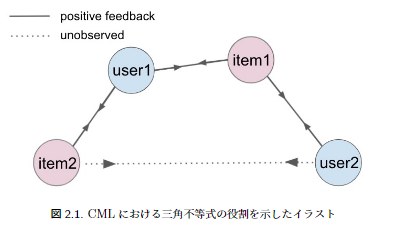
\includegraphics[width=0.8\textwidth]{CMLにおける三角不等式の役割を示したイラスト.png}
  \caption{CMLにおける三角不等式の役割を示したイラスト}
\end{figure}

よって、インタラクションを観測していないユーザーアイテムペアの関係性でも、潜在的にインタラクションが起きやすいユーザーアイテムペアの距離を近づける機構があることが確認できる。

膨大な組み合わせとなる$\mathcal{S, D}$に対して$\mathcal{L}^{\text{cml}}$をの大域的最適解を求めることは現実的に難しい。そのため、1)ミニバッチのサンプリング、2)損失の計算、3)パラメータの更新、を損失が収束するまで繰り返すことでCMLを実行する。いわゆる確率的勾配降下法である。

また、ミニバッチのサンプリングは\textbf{ポジティブサンプリング}と\textbf{ネガティブサンプリング}の2つに分かれる。ポジティブサンプリングは、ポジティブなフィードバック$Y_{u,i} = +1$を持つユーザーアイテムペア$(u,i)$を$S$から決められた個数ランダムに抽出する。そのサンプルを$\mathcal{B} \subset \mathcal{S}$と表し、これをポジティブサンプルと呼ぶ。そして、$\mathcal{B}$に含まれる任意のユーザーアイテムペア$(u,i)$に対して、ユーザー$u$とポジティブなフィードバックをもたない$Y_{u,j} = -1$なるアイテム$j$を$\mathcal{D}_u$から決められた個数ランダムに抽出する。そのアイテムを$\mathcal{N}_{u,i} \subset \mathcal{D}_u$と表し、これをネガティブサンプルと呼ぶ。

サンプリングとパラメータ更新のイテレーションによる局所最適解の求解に合わせ、ミニバッチの損失関数も修正される。
$$
  \mathcal{L}^{\text{batch}}(\Theta, \mathcal{B}, \{\mathcal{N}_{u,i}\}_{(u,i) \in \mathcal{B}}) = \sum_{(u,i) \in \mathcal{B}} [1 + d(\mathbf{v_u}, \mathbf{v_i})^2 - \underset{j \in \mathcal{N}_{u,i}}{\min} d(\mathbf{v_u}, \mathbf{v_j})^2]_+
$$

先ほどの式との大きな相違点は、各ユーザー$u$についてポジティブなフィードバックを持たないアイテム$j$に関する損失についてである。こちらではユーザー$u$に対して最近傍に位置するネガティブアイテム$j$に対する損失のみを考慮する。これは、ユーザーに対して遠くに位置したネガティブアイテムをさらに遠ざけることよりも、より近くに位置したネガティブアイテムを遠ざけることを重視した方がより良い解が得られる直感を利用した形式である。

\subsubsection*{2.3 ノイズラベルを用いた教師あり学習(信頼学習)}

入力$x_d$に対してラベル$y \in \{ 1, 2, ... M\}$を付与するのはかなりコストになる。そのためクラウドソーシングのような手法でラベル付けを行うこともあり、この場合はデータ作成の質が低くなる。また、医療分野などではCTR画像から専門家が病気のラベリングをすることがあるが、専門家でさえもその精度は完璧ではない。これらが\textbf{ノイズラベル問題}である。

ノイズラベル問題への対策は、近年研究がされているが、推薦システムに応用が可能と考えられる手法は大きく2つ存在する。

1つは、前節でも紹介した\textbf{重みづけをベースとした手法}である。この方法は、事前もしくは学習中にデータの信頼度を推定し、損失関数もしくは確率的勾配降下法におけるミニバッチのサンプリング確率を疎の信頼度を元に重みづけするという手順をとる。これは比較的容易に実装可能である。

2つ目が\textbf{クリーニングをベースとした手法}である。この方法は、事前にデータの信頼度を推定し、信頼できないデータを除去したうえで通常の教師あり学習を行う。特にNorthcuttらは教師あり学習の分類予測タスクにおける汎用的な方法として、信頼学習(Confident Learning)を提案した[32]。

\textbf{信頼学習}

特徴量$\bm{x} \in \mathcal{R}^d$およびノイズを含むラベル$\hat{y} \in \{ 1, 2, ... M \}$からなるデータセット$\mathcal{D} = \{ (\bm{x}_i, \hat{y}_i) \}_{i=1}^N$を用いて、新たな入力$\bm{x}_{\text{new}}$の各ラベル$j \in \{ 1, 2, ... M\}$への所属確率$p(y_{\text{new}} = j | \bm{x}_{\text{new}})$を予測するタスクを考える。すなわち、任意のパラメータ$\Theta$でパラメータ化された関数$f(\bm{x}|\Theta), f:\mathcal{R}^d \to \mathcal{R}^M$を用いて、
$$
  p(y_{\text{new}} = j | \bm{x}_{\text{new}}) \approx \hat{p}(y_{\text{new}} = j | \bm{x}_{\text{new}}) = \text{Softmax}_j(f(\bm{x}_{\text{new}} | \Theta)), j=1,...,M
$$

となるよう$\Theta$を最適化する。ただし、$\text{Softmax}_j$は入力ベクトル$\bm{z} \in \mathcal{R}^M$の各要素$z_j,(j=1,...,M)$を用いて、$j$番目のラベルへの所属確率$p_j = \frac{\exp(z_j)}{\sum_{k=1}^M \exp(z_k)}$に変換する関数である。




\section{ノイズラベルを用いた教師あり学習 (信頼学習)}
一般に、ある入力 $x\in\mathbb{R}^{d}$ とそのラベル $y\in\{1,2,...,M\}$ からなるデータセット $\{(x_{i},y_{i})\}_{i=1}^{N}$ を用いて $y\approx f(x)$ なる分類モデル fを学習し、未観測のデータ $x_{new}$ に付与されるラベル $y_{new}$ を予測するタスクを教師あり学習における多クラス分類と呼ぶ、その代表的な例が画像分類である。例えば、犬の画像と猫の画像のベクトル表現を大量に用いて、新たに入力される画像が「犬」 ラベルか 「猫」 ラベルかを予測する。近年では深層学習による手法を中心に世界中で研究され、一定の成果を挙げている。

しかしながら、実務上の課題としてノイズラベル問題が指摘されている。教師あり学習は、多くのラベル付きデータを要する。先に挙げた画像分類の例では想像に難くないが、タスクによっては人が1データずつ目で判断しなくてはならないなど、このラベルを収集するコストが大きい場合がある。このような場合、データ収集コスト削減のため、クラウドソーシングなどによって不特定多数の人にデータ作成を依頼するケースもあり、そのデータ作成の質が低いケースも散見される、また、専門家でもそもそもラベルを与えることが難しい場合もある。例えば医療分野において、CTR画像から病気を発見する応用が提案されているが、医者でも全ての画像に完全に正しく病気を割り当てられないと言われている。これらのような状況において教師あり学習を行う際に注意すべき点がノイズラベル問題である。すなわち、それぞれのデータに与えられたラベルが必ずしも正解ではないということを無視すべきでないという問題設定である。

このようなノイズラベル問題への対策は、実応用が進むにつれて近年研究がされている。特に、推薦システムにも応用が可能と考えられる手法は大きく2つ存在する。

1つは、前節でも紹介した重み付けをベースとした手法である。この方法は、事前もしくは学習中にデータの信頼度を推定し、損失関数もしくは確率的勾配降下法におけるミニバッチのサンプリング確率をその信頼度をもとに重み付けするという手順をとる。これにより、ノイズでないとみなせるデータの誤差を重視して学習することができる。これは推薦システムにも比較的容易に実装可能であるため、前節で紹介した重み付き行列分解をはじめとするいくつかの既存研究が存在する。

2つ目が、クリーニングをベースとした手法である、この方法は、事前にデータの信頼度を推定し、信頼できないデータを除去した上で通常の教師あり学習を行う、特に、Northcuttら は教師あり学習の分類予測タスクにおける汎用的な方法として、信頼学習 (Confident learing) と呼ばれる手法を提案した \cite{32} 以下でその概要を示す。

\subsection{信頼学習(Confident Learning)}
特徴量 $x\in\mathbb{R}^{d}$ およびノイズを含むラベル $\tilde{y}\in\{1,2,...,M\}$ からなるデータセット $\tilde{\mathcal{D}}=\{(x_{i},\tilde{y}_{i})\}_{i=1}^{N}$ を用いて、新たな入力 $x_{new}$ の各ラベル $j\in\{1,2,...,M\}$ への所属確率 $p(y_{new}=j|x_{new})$ を予測するタスクを考える。すなわち、任意のパラメータでパラメータ化された関数 $f(x|\Theta),f:\mathbb{R}^{d}\rightarrow\mathbb{R}^{M}$ を用いて、
$$P(Y_{new}=j|X_{new}) \approx\hat{p}(Y_{new} = j|x_{new}) = \text{Softmax}_{j}(f(x_{new}|\Theta)), j = 1,..., M$$
となるよう$\Theta$を最適化する。ただし、$\text{Softmax}_{j}$は、入力ベクトル $z\in\mathbb{R}^{M}$ の各要素 $z_{j},(j=1,...,M)$ を用いて、$j$番目のラベルへの所属確率 $p_{j}=\frac{\exp(z_{j})}{\sum_{j'=1}^{M}\exp(z_{j'})}$ に変換する関数である。ただし、必ずしも$\tilde{y}$が真のラベル $y$ とは異なることに注意する。信頼学習は、このような設定において、$\tilde{\mathcal{D}}$や$f$の形状および最適化の手順に依らず、以下の手順によって実行される。

\begin{enumerate}
    \item まず単純にノイズデータ$\tilde{\mathcal{D}}$を用いてモデル $\tilde{f}(x|\tilde{\Theta})$ を学習する。
    \item 各データ $i=1,...,N$ および各ラベル $j=1,...,M$ について、モデル $\tilde{f}$ を用いて以下で定義されるノイズ率 $\rho_{j,x_{i}}$ を計算する。
    \begin{align}
        \rho_{j,x_{i}}&=\hat{p}(y=j|x_{i})-\hat{p}(y=\tilde{y}_{i}|x_{i}) \label{eq:2.6} \\
        &= \text{Softmax}_{j}(f(x_{i}|\Theta))-\text{Softmax}_{\tilde{y}_{i}}(f(x_{i}|\Theta)) \label{eq:2.7}
    \end{align}
    \item 各ラベル $j=1,...,M$ について、 $\rho_{j,x}$ が大きいデータ $(x_{i},\tilde{y}_{i})$ を$\tilde{\mathcal{D}}$から除外し、データセット $\mathcal{D}'$を作成する。
    \item $\mathcal{D}'$ を用いてモデル fを学習する。
\end{enumerate}
これらの手順を要約すると、ノイズを含むデータで学習・予測した各ラベルの所属確率をもとにノイズ率を算出しデータをクリーニングする方法と言える。従ってこの方法は、ノイズラベルを用いて各ラベルへの所属確率が推定可能であれば適用が可能であると言える。よって、推薦システムでもノイズラベル $Y_{u,i}$ の所属確率 $P(Y_{u,i}=+1),P(Y_{u,i}=-1)$ を推定することで、これと類似した方法を適用することができると考えられる。

以上のように、推薦システムに適用可能と考えられるノイズへの対応は、1) 重み付け 2) クリーニングと2種類存在するが、これらには情報損失とノイズへの脆弱性の間でトレードオフの関係がある、重み付けは、データを切り捨てないため情報損失が少ないが、一定確率でノイズが含まれてしまう。一方で、クリーニングは、データ削除割合を適切に定めれば確実にノイズのあるデータが削除され、ノイズのないデータも失われてしまい、学習の効率性を損なう可能性がある。これらは、状況や問題に応じて取るべき手法が異なると言える。





\end{document}